\documentclass{beamer}

% Top-aligning columns within a top-aligned frame
% https://tex.stackexchange.com/questions/16447/beamer-top-aligning-columns-within-a-top-aligned-frame
\makeatletter
\newenvironment{myitemize}{%
   \setlength{\topsep}{0pt}
   \setlength{\partopsep}{0pt}
   \renewcommand*{\@listi}{\leftmargin\leftmargini \parsep\z@ \topsep\z@ \itemsep\z@}
   \let\@listI\@listi
   \itemize
}{\enditemize}
\makeatother  

\usepackage[USenglish]{babel}
\usepackage[utf8]{inputenc}
\usepackage{amssymb, amsmath}
\usepackage{bm}
\usepackage{color}
\usepackage{tikz}
\usepackage{url}
\hypersetup{
    colorlinks,
    citecolor=blue,
    filecolor=blue,
    linkcolor=blue,
    urlcolor=blue
}

\usetheme{Warsaw}
\setbeamertemplate{headline}{}
\newcommand*\oldmacro{}%
\let\oldmacro\insertshorttitle%
\renewcommand*\insertshorttitle{%
  \oldmacro\hfill%
  \insertframenumber\,/\,\inserttotalframenumber}
  

\bibliographystyle{apalike}
% make bibliography entries smaller
%\renewcommand\bibfont{\scriptsize}
% Now get rid of all the colours
\setbeamercolor*{bibliography entry title}{fg=black}
\setbeamercolor*{bibliography entry author}{fg=black}
\setbeamercolor*{bibliography entry location}{fg=black}
\setbeamercolor*{bibliography entry note}{fg=black}

% and kill the abominable icon
\setbeamertemplate{bibliography item}{}

\begin{document}
\title{Born Again Neural Networks}  
\author{Radek Bartyzal}
\date{Date TBA} 
\institute{Let's talk ML in Prague}

\frame{\titlepage} 

\begin{frame}{Prior work}


\begin{block}{Ensembles}
Diverse models with similar validation performances can be often be combined to achieve predictive
power superior to each of the constituent models. \cite{cit:ensembles}
\end{block}

\begin{block}{Born again trees}
Learn a single tree that is able to recover the performance of a multiple-tree predictor. \cite{cit:bat}
\end{block}

\begin{block}{Knowledge distillation = model compression}
Transfer knowledge acquired by a learned
teacher model to a new simpler student model. \cite{cit:distill}
\end{block}



\end{frame}
%--------- END Frame 1 -------------

\begin{frame}[t]{Knowledge distillation}

\begin{columns}[t]
\begin{column}{0.5\textwidth}
Teacher
\begin{itemize}
\item high-capacity model
\item good performance
\end{itemize}
\end{column}

\begin{column}{0.5\textwidth}
Student
\begin{itemize}
\item more compact model
\item not as good performance as the teacher but better than if it was trained without it
\end{itemize}
\end{column}

\end{columns}

\vfill
By transferring knowledge, one hopes to benefit from the student’s
compactness while suffering only minimal degradation in performance.

\end{frame}
%--------- END Frame 2 -------------

\begin{frame}{Knowledge distillation}

Teacher produces soft targets = probabilities of incorrect classes = the key to generalization outside of the training dataset.

\vfill

Training student = minimize weighted average of:

\begin{itemize}
\item cross entropy with the soft targets
\item cross entropy with the hard targets = labels
\end{itemize}


\end{frame}
%--------- END Frame 3 -------------

\begin{frame}{Knowledge distillation results}

\begin{figure}[h]
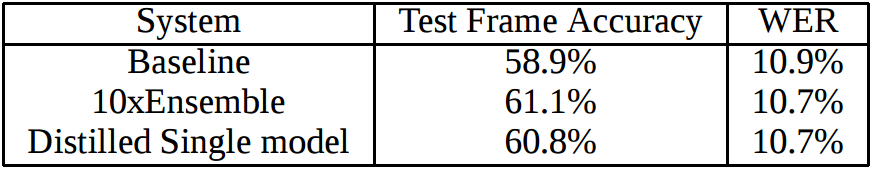
\includegraphics[width=\textwidth]{img/distilled_result}
\caption{DNN acoustic models used in Automatic Speech Recognition. \cite{cit:distill}}
\end{figure}

\end{frame}
%--------- END Frame 4 -------------
\begin{frame}{Born Again Networks (BANs)}

\begin{itemize}
\item not compressing models
\item students are parameterized identically to their parents
\item students outperform teachers
\item knowledge transfer between dense networks and residual
networks of similar capacity
\end{itemize}

\vfill

\begin{figure}[h]
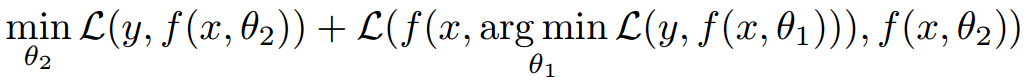
\includegraphics[width=\textwidth]{img/BAN_loss_func}
\caption{BAN loss function adding Kullback–Leibler divergence between the new model’s outputs and the outputs of the original model. \cite{cit:ban}}
\end{figure}

\end{frame}
%--------- END Frame 5 -------------
\begin{frame}{BAN Ensembles}

Apply BANs sequentially with multiple generations of knowledge transfer. In
each case, the $k$-th model is trained, with knowledge transferred from the $k-1$-th student:

\begin{figure}[h]
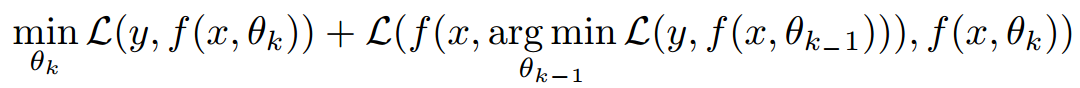
\includegraphics[width=\textwidth]{img/sequential_ban1}
%\caption{ \cite{cit:ban}}
\end{figure}

\begin{block}{Born Again Network Ensemble (BANE)}
Averaging the prediction of multiple generations of BANs.
\end{block}
 

\end{frame}
%--------- END Frame 6 -------------
\begin{frame}{DenseNets reminder: Dense block }

\begin{figure}[h]
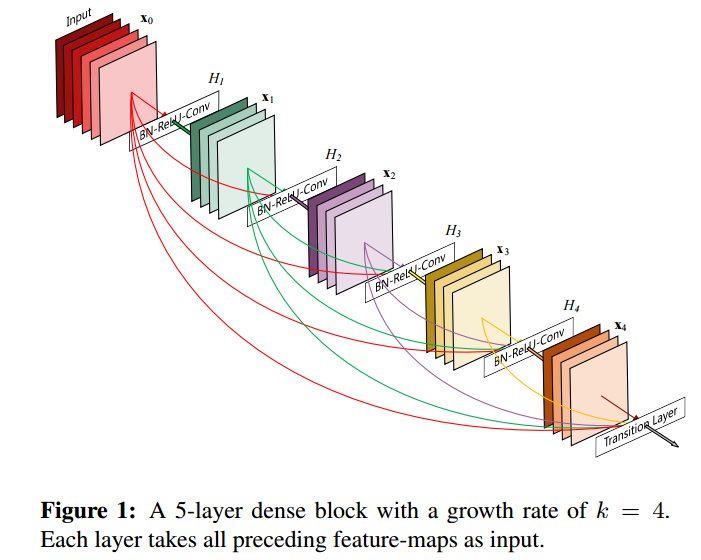
\includegraphics[width=\textwidth]{img/denseBlock}
%\caption{Dense block \cite{cit:ban}}
\end{figure}

\end{frame}
%--------- END Frame 7 -------------
\begin{frame}{DenseNets reminder: Deep DenseNet }

\begin{figure}[h]
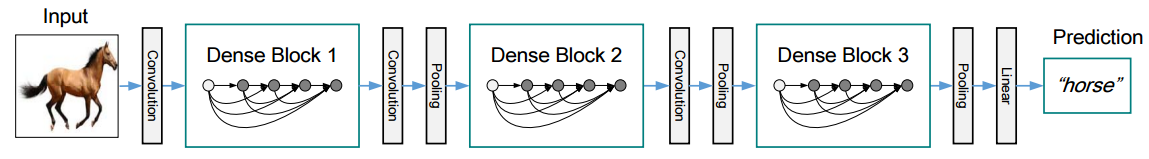
\includegraphics[width=\textwidth]{img/denseNet}
\caption{A deep DenseNet with three dense blocks. The layers between two adjacent blocks are referred to as transition layers and change
feature-map sizes via convolution and pooling. \cite{cit:densenet}}
\end{figure}

\end{frame}
%--------- END Frame 8 -------------
\begin{frame}{BAN DenseNets Experiments }

All experiments on: CIFAR-100 (100 classes each containing 600 32x32 colour images).

\begin{itemize}
\item DenseNet-BC-(depth)-(growth rate)
\item BAN-1/2/3 = sequential training by previous BAN-(k-1)
\item Ens*2/3 = ensembles of 2/3 BAN-x
\end{itemize}

\begin{figure}[h]
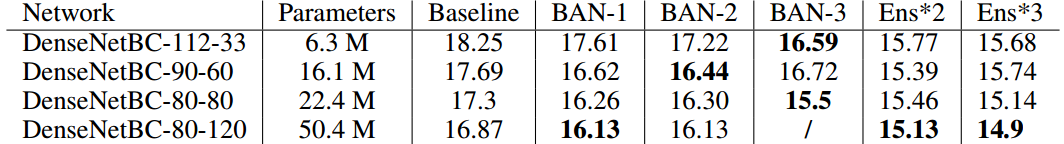
\includegraphics[width=\textwidth]{img/denseNet_experiment}
\caption{BAN training is clearly beneficial for DenseNets on CIFAR. \cite{cit:ban}}
\end{figure}

\end{frame}
%--------- END Frame 9 -------------
\begin{frame}{ResNets reminder}
\begin{figure}[h]
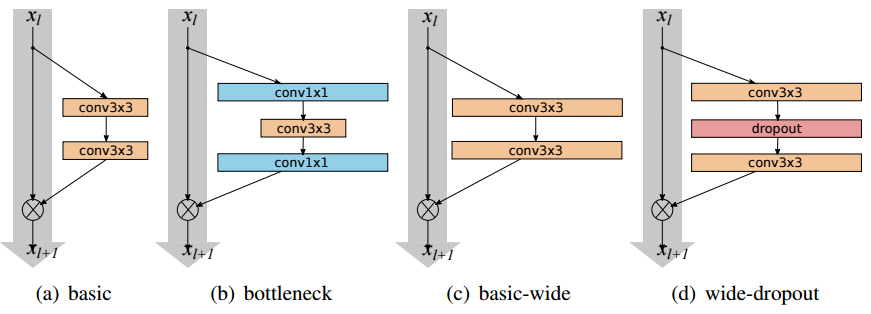
\includegraphics[width=\textwidth]{img/resnet_blocks}
\caption{Various residual blocks used in the paper. Batch normalization and ReLU precede
each convolution (omitted for clarity). \cite{cit:resnet}}
\end{figure}
\end{frame}
%--------- END Frame 10 -------------
\begin{frame}{BAN ResNets}
BAN-ResNets:
\begin{itemize}
\item trained by DenseNet 90-60 teacher
\item baseline = wide-ResNet28 \cite{cit:resnet}
\item tested multiple nets with different number of units per block
\item all benefit from BAN training
\end{itemize}

\vfill

BAN-ResNets outperform:
\begin{itemize}
\item traditional counterparts
\item equivalent ResNets trained without DenseNet teacher
\item their DenseNet teacher
\end{itemize}
\end{frame}
%--------- END Frame 11 -------------
\begin{frame}{BAN Results}

Single model non-ensemble SOTA on CIFAR 100 trained with SGD without any sort
of shake-shake regularization:
\begin{itemize}
\item BAN-3-DenseNet-80-80
\item 22M parameters
\item 15.5\% error 
\end{itemize}

\vfill

Ensemble SOTA under the same conditions:
\begin{itemize}
\item BAN-3-DenseNet-BC-80-120
\item 150M parameters
\item 14.9\% error 
\end{itemize}
\end{frame}

%--------- END Frame 12 -------------
\begin{frame}{Sources}

\begin{thebibliography}{0}

  \bibitem[1]{cit:ban} 1. Tommaso Furlanello et al. "Born Again Neural Networks." Workshop on Meta-Learning (MetaLearn 2017) at NIPS. Accessible from: \url{http://metalearning.ml/papers/metalearn17_furlanello.pdf}
  
  \bibitem[2]{cit:stat} 2. Breiman, Leo. "Statistical modeling: The two cultures (with comments and a rejoinder by the author)." Statistical science 16.3 (2001): 199-231. Accessible from: \url{https://projecteuclid.org/download/pdf_1/euclid.ss/1009213726\%20}
  
  \bibitem[3]{cit:ensembles} 3. Hansen, Lars Kai, and Peter Salamon. "Neural network ensembles." IEEE transactions on pattern analysis and machine intelligence 12.10 (1990): 993-1001.
\end{thebibliography}

\end{frame}


\begin{frame}{Sources}

\begin{thebibliography}{0}
  \bibitem[4]{cit:bat} 4. Breiman, Leo, and Nong Shang. "Born again trees." ps (1996). Accessible from: \url{https://www.stat.berkeley.edu/~breiman/BAtrees.pdf}
  
  \bibitem[5]{cit:distill} 5. Hinton, Geoffrey, Oriol Vinyals, and Jeff Dean. "Distilling the knowledge in a neural network." arXiv preprint arXiv:1503.02531 (2015). Accessible from: \url{https://arxiv.org/pdf/1503.02531.pdf}
  
  \bibitem[6]{cit:densenet} 6. Huang, Gao, et al. "Densely connected convolutional networks." arXiv preprint arXiv:1608.06993 (2016). Accessible from: \url{https://arxiv.org/pdf/1608.06993.pdf}
  
  \bibitem[7]{cit:resnet} 7. Zagoruyko, Sergey, and Nikos Komodakis. "Wide residual networks." arXiv preprint arXiv:1605.07146 (2016). Accessible from: \url{https://arxiv.org/abs/1605.07146}
\end{thebibliography}

\end{frame}
 
 
 
\end{document}
